\documentclass[10pt,journal,compsoc]{IEEEtran}

\usepackage[pdftex]{graphicx}    
\usepackage{cite}
\hyphenation{op-tical net-works semi-conduc-tor}
\usepackage{mathtools}
\graphicspath{ {../images/} }

\begin{document}

\title{Robo Nano Degree: Localization Project }

\author{Manuel Huertas L\'opez}

\markboth{Localization project, Robotics Nanodegree Program, Udacity}%
{}
\IEEEtitleabstractindextext{%

\begin{abstract}

This project involves to accurately localize a mobile robot insided a provided map in Gazebo and RViz simulation enviroments. The goal includes to build a robot model in Gazebo and utilize packages like AMCL and the Navigation Stack to succefully identifed the position of the robot in the world. As a final test the robot will be commaned to a specific location and the navigation stack will determinate the route to follow. As part of the work it is neccessary to explore, add, and tunning specific parameters corresponding to each package to achieve the best possible localization result.


\end{abstract}


\begin{IEEEkeywords}
Robot, Udacity, Monte Carlo Filter, Kalman Filter, Localization.
\end{IEEEkeywords}}


\maketitle
\IEEEdisplaynontitleabstractindextext
\IEEEpeerreviewmaketitle
\section{Introduction}
\label{sec:introduction}

\IEEEPARstart{M}{obile} robot localization is the process to determine where a robot is located with respect to its environment. It is one of the fundamental parts required by a robot to achieve autonomous navigation.

In its simplest form, position tracking, the initial robot pose is known and it is only necessary to correct incremental errors in the robot odometry. More challenging is the global localization problem, where the robot must determinate its initial pose by itself. Finally, in the kidnapped robot problem the robot is tele-ported to other position without beaing told. The kidnapped problem can be used to teach the robot how to recover from a system fail, where the robot prevoius knowlegde is complety lost.

Localization can be used in so many applications ranging from robots to clean the floors to robot to explore other planets.

The localization algorithms must overcome some difficulties like the errors in the sensor measurement: both odometry sensor and sensor to measure the distances in the scene. The algorithm used for the project use bayesian probability to evaluate the probability of a hipothesis, where the robot is located, base on the observation of the environment.


\section{Background}


At this stage, you should begin diving into the technical details of your approach by explaining to the reader what are the characteristics of the filters, what localization method was chosen, and the reason that it was selected (i.e. particle filters). 
This should be factual and authoritative, meaning you should not use language such as "I think this will work" or "Maybe Monte Carlo Localization with these parameters is better...". Instead, focus on items similar to, "Adaptive Monte Carlo Localization was chosen because..."
Provide a sufficient background into the scope of the problem technologically while also identifying some of the current challenges in robot localization and why the problem domain is an important piece of robotics.\cite{lamport1994latex}

\subsection{Kalman Filters}

Kalman filter was invented by Rudolf Kalman and it was used to solve non-linear problem of the trajectory estimation of the Apollo program. It helped to the Apollo to orbit around the moon. 

Kalman filter is an estimation algorithm used to estimate the value of a variable as the data is being collected. It can take data, from sensors, with a lot of uncertainty or noise in measurements and provide a very accuate estimate of the real value. It can do it fast and without needing too much computer power. 

Kalman filter can be used for local localization problem where both the odometry and the movement contains a lot of noise and uncertains. The Kalman filter is continuosly iterating two steps: measurement update where the measurement is used to update the robot's position, and state prediction where the information about the current state is used to predict the future pose. At the beginning an initial guess is used. After a few iterations the measurement converge to the real value.

The Kalma filter assumes a Gaussian distribution of the noise an uncertaions and it is only valid for linear system.

\begin{align}
P(x) = \frac{1}{{\sigma \sqrt {2\pi } }}e^{{{ - \left( {x - \mu } \right)^2 } \mathord{\left/ {\vphantom {{ - \left( {x - \mu } \right)^2 } {2\sigma ^2 }}} \right. \kern-\nulldelimiterspace} {2\sigma ^2 }}}
\end{align}

Nevertheless, a variation of the algorithm, the Extended Kalman filter can be used for nonlinear system. The EKF linearize the original nonlinear filter dynamics around the previous estimates.

\subsection{Particle Filters}

The Monte Carlo localization is the most popular localization algorithm in robotics. It can solve the local an global localization problems. The robot will navigate inside a known map collecting information using range sensors. MCL uses these sensor measurement to keep track of the robot pose. 

In MCL a set of particles are initially spread randomly and uniformly throughout the entire map. These virtual particles represents the hypothesis of whre the robot might be. In a 2D map, each particle has got a position , orientation and weight value. The importance of the particle depends on the weight, the bigger the more accurate and during the resamping process they are more likely to survive. After several iterations of the Monte Carlo algorithm the particles will converge and estimate the robot's pose.

The MCL uses a Bayes filtering to estimate a probability density over the state space conditioned by the measurement, this probability density is called belief:

\begin{align}
Bel(X{t}) = P(X{t} |Z{1}...{t} )
\end{align}

X{t} are the state of the robot and Z are the measurement from time 1 up to time {t}. The belief is estimated recursivelly, the initial guess uses a randomly and uniformly distribution over the entire map.

The MCL has got two sections. In every iteration the algorithm takes the previous belief, the actuaion commands and the sensor measurement as input. The hypothetical state is computed whenever the robot moves, the particles weight are computed using the latest sensor measurement. Secondly the particles with high probability, the ones that fetch better the measurement reading, will survive and the others will die. The algorithm will output the new beliefe of the next iteration. After few iteration the survivors particles will represent the real robot's pose.


\subsection{Comparison / Contrast}

MCL presents many adventages over EFK:

\begin{itemize}
\item MCL is easier to program than EFK 
\item In the EFK algorithm the noise error and uncertaions must follow a gaussian distribution, MCL is not tied to the measure noise distribution.
\item MCL can control the computational memory and resolution of the solution by changing the number of particles distributed.
\end{itemize} 

In the present work the particle filter is going to be used.


\section{Simulations}
This section should discuss the performance of robots in simulation. Items to include are the robot model design, packages used, and the parameters chosen for the robot to properly localize itself. The information provided here is critical if anyone would like to replicate your results. After all, the intent of reports such as these are to convey information and build upon ideas so you want to ensure others can validate your process.
You should have at least two images here: one that shows your standard robot used in the first part of the project, and a second robot that you modified / built that is different from the first robot. Remember to watermark all of your images as well. 

\subsection{Achievements}
You should describe what you achieved for localization in the project with the benchmark model and your own model. Includes charts and graphs show how parameters affect your performance. 

% Robot Models
\subsection{Benchmark Model}


\subsubsection{Model design}
The Robot's design considerations should include: the size of the robot, the layout of sensors. This information can be shown in the form of a chart / table.

\subsubsection{Packages Used}
The packages used in the project should be specified as well as the topics received and published; the services it used and provided should also be addressed. 

\subsubsection{Parameters}
Localization parameters in the AMCL node should be described, as well as move\_base parameters in the configuration file. You should be able to clearly demonstrate your understanding of the impact of these parameters.

\subsection{Personal Model}
% ditto
\subsubsection{Model design}

\begin{figure}[t]
\centering
\subfigure{
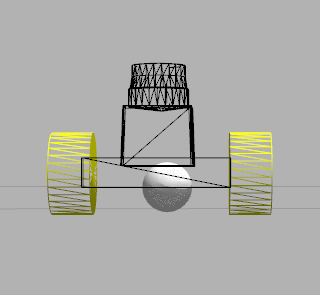
\includegraphics[width=.1\textwidth, height=0.15\textwidth]{robokoko-design-1}
}
\subfigure{
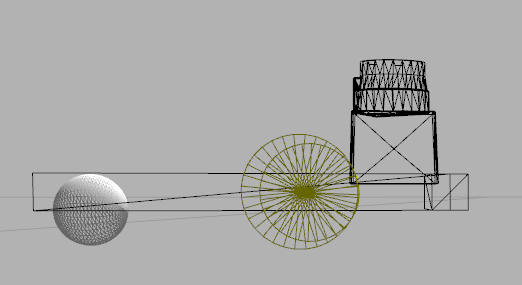
\includegraphics[width=.2\textwidth, height=0.15\textwidth]{robokoko-design-2}
}
\subfigure{
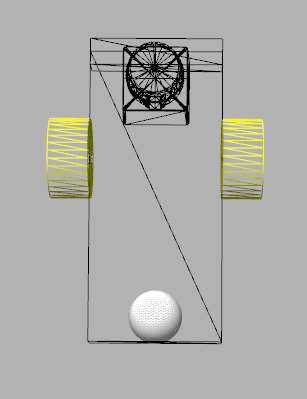
\includegraphics[width=.1\textwidth, height=0.15\textwidth]{robokoko-design-3}
}
\caption{blablabla}
\label{fig:whatever}
\end{figure}

\subsubsection{Packages Used}
\subsubsection{Parameters}


\section{Results}
Present an unbiased view of your robot's performance and justify your stance with facts. Do the localization results look reasonable? What is the duration for the particle filters to converge? How long does it take for the robot to reach the goal? Does it follow a smooth path to the goal? Does it have unexpected behavior in the process? \\
For demonstrating your results, it is incredibly useful to have some watermarked charts, tables, and/or graphs for the reader to review. This makes ingesting the information quicker and easier.

\subsection{Localization Results}
\subsubsection{Benchmark}
\subsubsection{Student}

\subsection{Technical Comparison} % only facts
Discuss the difference of the layout, parameters, performance etc. between the benchmark robot and your robot. It is acceptable for your custom robot to perform worse than the provided robot. The focus is on learning and understanding, not performance. 

\section{Discussion}
This is the only section of the report where you may include your opinion. However, make sure your opinion is based on facts. If your robot performed poorly, make mention of what may be the underlying issues. If the robot runs well, which aspects contribute to that? Again, avoid writing in the first person (i.e. Do not use words like "I" or "me"). If you really find yourself struggling to avoid the word "I" or "me"; sometimes, this can be avoid with the use of the word “one”. As an example: instead of : "I think the robot cannot localize itself because the sensor does not provide enough information for localization" try: "one may believe the localization performance is poor because the sensor layout is not able to provide enough information for localization". They say the same thing, but the second avoids the first person. 

\subsection{Topics}
\begin{itemize}
\item Which robot performed better?
\item Why it performed better? (opinion)
\item How would you approach the 'Kidnapped Robot' problem?
\item What types of scenario could localization be performed?
\item Where would you use MCL/AMCL in an industry domain?
\end {itemize}

\section{Conclusion / Future work}
This section is intended to summarize your report. Your summary should include a recap of the results, did this project achieve what you attempted, how would you deploy it on hardware and how could this project be applied to commercial products? 
For Future Work, address areas of work that you may not have addressed in your report as possible next steps. This could be due to time constraints, lack of currently developed methods / technology, and areas of application outside of your current implementation. Again, avoid the use of the first-person.

\subsection{Modifications for Improvement}
Examples:
\begin{itemize}
\item Base Dimension
\item Sensor Location
\item Sensor Layout
\item Sensor Amount
\end{itemize}

\subsection{Hardware Deployment}
\begin{enumerate}
\item What would need to be done?
\item Computation time/resource considerations?
\end{enumerate}



\bibliography{bib}
\bibliographystyle{ieeetr}

\end{document}